% /Users/pikachu/books/payments-book/src/parts/part4/ch20-compliance-aml.tex
\chapter{Комплаенс и AML}
\label{ch:compliance-aml}
\margintoc

\begin{kaobox}[title=Что вы узнаете из этой главы]
  Комплаенс в платёжном бизнесе работает как операционная функция:
  на входе клиента, на каждом этапе транзакции и после её завершения.
  Здесь разберём, что требует \law{115-ФЗ} от платёжного оператора, как устроены
  проверки клиента и мерчанта, где ставится санкционный скрининг,
  почему ложноположительные совпадения надо считать отдельно и
  чему учит индустрию кейс QIWI.
\end{kaobox}

В платёжном бизнесе комплаенс редко начинается с громкого инцидента.
Чаще всё решает будничный вопрос: кого именно мы сейчас подключаем,
что уже знаем об этом клиенте или мерчанте и в какой момент обязаны
остановить операцию, даже если бизнесу хочется провести её быстрее.
Из этого вопроса и вырастает весь конвейер главы: сначала
онбординг, потом проверка по спискам и профилям риска, затем
наблюдение за поведением после подключения, а при необходимости
эскалация и отчётность. Комплаенс поэтому нельзя сводить к
формальному чек-листу. Для платёжного продукта это часть рабочего
механизма, которая должна срабатывать внутри реального потока
операций, а не только красиво выглядеть в отчёте для регулятора.

\section{115-ФЗ и платёжный бизнес}
\label{sec:compliance-115fz}

\law{115-ФЗ} -- Федеральный закон \enquote{О противодействии
легализации (отмыванию) доходов, полученных преступным путём, и
финансированию терроризма} -- задаёт базовую рамку AML-контроля в
России \sidecite{fz-115}. Для платёжного оператора его смысл очень
практичен: пока клиент ещё не прошёл проверку, с его операцией
нельзя обращаться как с полностью доверенной. Закон раскладывает
эту задачу на три обязанности: знать клиента, наблюдать операции и
при формальных основаниях блокировать средства. Скорость здесь не
даёт права отключать осторожность. AML встроен в сам продукт, а не
вынесен во внешний формальный контур.

Первая обязанность касается идентификации. Закон различает
упрощённую, стандартную и полную идентификацию. Для оператора
это значит, что на одних регистрационных данных далеко не уедешь:
в одних сценариях достаточно упрощённой проверки, в других нужна
документальная верификация, а в самых чувствительных -- более
жёсткая процедура. Конкретные пороги и условия зависят от вида
операции и регулярно меняются, поэтому в печатной версии лучше
не привязываться к цифре, которая завтра может устареть.

Вторая обязанность связана с мониторингом. Оператор должен замечать
операции, которые подпадают под критерии обязательного контроля,
и отправлять сведения в Росфинмониторинг. Но этим задача не
ограничивается: надо ловить и те операции, которые формально ещё не
описаны в законе, но выбиваются из нормального профиля клиента по
поведению или по контексту. По форме эта система проста -- нужны
регламент, поток данных, маршрут проверки и понятное решение по
результату. На практике всё сложнее: если контроль настроен
формально, он либо ничего не увидит, либо захлебнётся в ложных
срабатываниях.

Третья обязанность -- заморозка средств. Если клиент или бенефициар
оказывается в перечнях лиц, связанных с терроризмом или экстремизмом,
оператор обязан немедленно остановить операции и сообщить об этом
в Росфинмониторинг \sidecite{fz-115}. И здесь важно не перепутать
скорость и осторожность: для AML промедление иногда опаснее
жёсткости.

Связь с лицензированием прямая. Банк России при надзоре за
оператором платёжной инфраструктуры проверяет не только формальные
правила, но и то, есть ли в компании рабочая AML-система,
обученные сотрудники и понятный маршрут обработки кейсов. \law{115-ФЗ}
задаёт не абстрактную добродетель, а конкретную операционную
обязанность. Локальный вывод здесь простой: AML-контур начинается
раньше первой спорной операции. Он определяет, кого продукт вообще
готов впустить и на каких условиях готов продолжать работу.

\section{KYC при онбординге физлиц}
\label{sec:compliance-kyc}

Что именно нужно знать о клиенте в момент первого контакта? Для
физлица KYC (Know Your Customer) начинается не с анкеты как таковой,
а с вопроса о степени доверия: можем ли мы считать этого человека
тем, за кого он себя выдаёт, и какой риск берём на себя, открывая
ему следующий уровень сервиса. В платёжном приложении это выглядит
очень приземлённо: после регистрации оператор решает, какие лимиты
оставить сразу, а какие открывать только после дополнительной
проверки. Поэтому KYC удобнее мыслить не как одно действие, а как
лестницу уровней доверия.

Обычно эта лестница идёт от регистрации по номеру телефона к
упрощённой идентификации через государственные сервисы, затем к
документальной проверке паспорта и, наконец, к более строгой
процедуре для чувствительных сценариев. На нижнем уровне у клиента
меньше прав и жёстче лимиты, на верхнем -- больше возможностей, но
и больше уверенности со стороны оператора. Автоматизация делает вход
быстрее, однако не отменяет базовой обязанности проверять качество
данных: ошибка на входе редко остаётся локальной. Поэтому KYC почти
всегда балансирует между удобством и точностью.

Практический набор проверок здесь вполне земной: сверка документов
по государственным источникам, проверка по перечням
Росфинмониторинга и санкционным спискам, а также выявление
политически значимых лиц (ПЭП).

\begin{kaobox}[title={Определение: Политически значимое лицо (ПЭП)}, colback=blue!4, colbacktitle=blue!15]
  ПЭП -- это человек, который занимает или занимал значимую
  публичную должность, а также его близкие родственники и
  связанные лица. Для ПЭП применяют усиленную проверку
  (enhanced due diligence, EDD), потому что риск здесь выше
  среднего: доступ к публичной власти всегда создаёт
  дополнительный контекст.
\end{kaobox}

Итак, KYC для физлица устроен как постепенное наращивание доверия,
а не как разовая формальность на входе. Чем чувствительнее сценарий
и выше риск, тем меньше система может полагаться на самодекларацию
и тем больше ей нужны внешние подтверждения. У мерчанта задача
сложнее ещё на один слой: там приходится проверять не только
человека, но и сам бизнес как действующую конструкцию.

\section{KYB при онбординге мерчантов}
\label{sec:compliance-kyb}

Чем проверка компании отличается от проверки физлица? Прежде всего
тем, что у юридического лица нужно оценить не только личность, но и
деловую конструкцию: структуру собственности, реальный вид
деятельности, возвраты, спорные операции и риск использования
бизнеса как транзитной оболочки. Платформа, которая подключает
нового продавца, должна понять не просто название компании, а то,
кто за ней стоит и как она действительно зарабатывает. Поэтому KYB
(Know Your Business) собирает регистрационные данные, владельцев,
хозяйственную модель и платёжное поведение в единый профиль риска.
Это не бумажная церемония, а условие безопасного приёма денег.

Базовый пакет документов включает выписку из реестра, данные
директора и учредителей, сведения о бенефициарном владельце
(ultimate beneficial owner, UBO), банковские реквизиты и описание
бизнеса. Если структура владения не сходится, а сайт не похож на
заявленный вид деятельности, вопросы должны возникнуть сразу.
Проверка строится на сопоставлении официальных данных с тем, как
бизнес выглядит в реальности. Но формально чистая компания вполне
может оказаться рискованной на практике. Именно поэтому KYB нельзя
заканчивать папкой с документами: после онбординга его приходится
постоянно сверять с живым поведением бизнеса.

Проверка MCC особенно важна. Некоторые категории мерчантов по самой
своей природе рискованнее других: азартные игры, контент для
взрослых, туристические услуги, обмен криптоактивов и другие
чувствительные сегменты. Эквайеры обычно вводят для них особые
условия и ограничения \sidecite{visa-core-rules}. Подмена MCC -- это
попытка спрятать реальный профиль бизнеса под более мягкой
категорией. Если заявленная категория не сходится с фактической
деятельностью, платёжный поток лучше останавливать до выяснения.

Модель платёжного фасилитатора (payment facilitator, PayFac)
меняет место ответственности, но не смысл проверки. Платформа
может подключать субмерчантов быстрее, но за это она платит
собственными процедурами KYB и более плотным мониторингом.
Иначе скорость подключения превращается в скорость накопления риска.

Локальный вывод здесь такой: KYB нужен не для того, чтобы собрать
идеальную папку документов, а для того, чтобы понять, совпадает ли
юридический фасад бизнеса с его реальным платёжным поведением.

\begin{kaobox}[title=На практике]
  Если вы проверяете мерчанта, смотрите не только на документы, но и
  на то, как бизнес выглядит на сайте, какие у него товары, как
  устроены возвраты и нет ли противоречия между заявленным MCC и
  фактической деятельностью. В KYB ошибка в одну сторону стоит
  регуляторного риска, а ошибка в другую -- лишнего отказа
  нормальному бизнесу.
\end{kaobox}

\begin{figure}
  \centering
  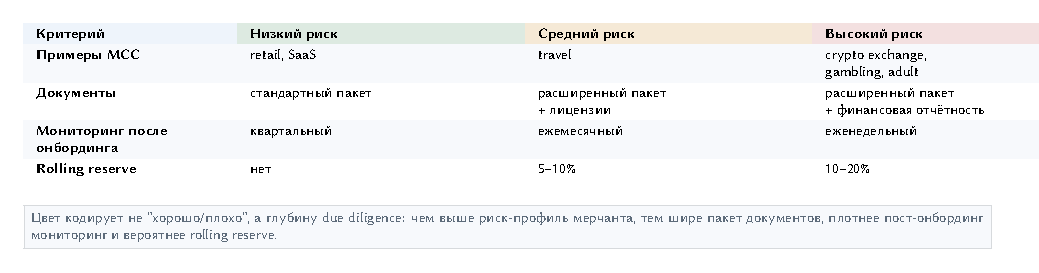
\includegraphics[width=\linewidth]{assets/figures/ch20-compliance-aml/compliance-kyb-risk.pdf}
  \caption{Чек-лист KYB по категориям риска.}
  \label{fig:compliance-kyb-risk}
\end{figure}

\section{Санкционный скрининг}
\label{sec:compliance-sanctions}

Санкционный скрининг -- это обязательный фильтр в тех точках, где
бизнес может вступить в отношения с запрещённым лицом или
юрисдикцией. Если клиент, бенефициар или контрагент попадает в
санкционный список, операцию нужно остановить до исполнения.
Проверка строится на сопоставлении имён, документов и реквизитов с
актуальными перечнями. Трудность в том, что списки длинные, имена
повторяются, а совпадение ещё не означает реальный риск. Поэтому
санкционный контроль должен быть точным, но не слепым.

Основные списки обычно включают OFAC SDN, сводный санкционный список ЕС,
санкционные списки ООН и внутренние перечни, с которыми оператор
работает по требованиям национального регулирования. Проверка
должна стоять минимум в четырёх местах: на онбординге, при каждой
значимой транзакции, при обновлении данных клиента и при обновлении
самих списков. Последний пункт особенно важен: новое имя появляется
сегодня, а проверить нужно и весь накопленный клиентский портфель.
Поэтому санкционный контроль требует не только онлайн-проверки, но
и ретроспективного прогона. Без него система видит новых клиентов,
но может пропустить старых.

Настоящая сложность начинается там, где скрининг работает в онлайне.
Если проверка тормозит авторизацию, бизнес неизбежно ищет
компромисс между скоростью и полнотой. Поэтому рабочая система
обычно строится на индексах в оперативной памяти и на чёткой
очереди эскалации: ручная проверка каждого совпадения здесь просто
не масштабируется. Проблема в том, что распространённые имена и
совпадения между кириллицей и латиницей порождают массу шума.
Важно не только находить подозрительные совпадения, но и быстро
разбирать ложные.

Управление ложноположительными совпадениями -- отдельная
операционная дисциплина. Типовой сценарий прост: система помечает
операцию как требующую проверки, сотрудник смотрит контекст, после
чего либо снимает блок, либо отправляет случай на эскалацию. Такой
маршрут должен быть формализован, иначе итог начнёт зависеть от
того, кто именно дежурит на смене. Если порог совпадения слишком
мягкий, команда утонет в шуме; если слишком жёсткий -- пропустит
риск. Санкционный скрининг заканчивается не на поиске имени, а на
дисциплине разбора срабатываний. И всё же даже хороший скрининг
решает только часть задачи: он помогает не впустить явный риск и
вовремя остановить операцию, но не заменяет наблюдение за тем, как
мерчант ведёт себя уже после подключения.

\section{Мониторинг мерчантов после подключения}
\label{sec:compliance-merchant-monitoring}

Почему мониторинг не заканчивается на онбординге? Потому что риск
меняется уже после подключения. Именно на этом отрезке возникают и
схемы типа bust-out, и попытки использовать мерчанта для отмывания:
пока профиль выглядит спокойно, система расслабляется, а потом
видит проблему слишком поздно. Поэтому защита должна отслеживать
изменения объёма, структуры чека, географии и доли возвратов. Один
спокойный месяц ничего не гарантирует на следующий; подключение --
это только начало наблюдения.

Поведенческие сигналы для расследования здесь вполне конкретны:
резкий рост оборота за короткое время, смена среднего чека,
нетипичная география клиентов, высокий процент возвратов и
спорных операций, несоответствие кода категории мерчанта реальной
деятельности. Ничего мистического в этом нет: это обычные правила
мониторинга транзакций, только применённые к мерчантскому профилю.
Но без контекста даже чистая статистика способна ввести в
заблуждение. Мониторинг мерчанта должен учитывать и цифры, и
деловую логику.

В промышленных системах это обычно выглядит как слой поверх
авторизационной базы: агрегаты по мерчанту, скользящие окна,
поиск выбросов и очередь кейсов для аналитиков. Если у мерчанта
внезапно растёт объём операций, команда должна увидеть это почти
сразу, а не ждать конца месяца. Смысл такой системы в том, что она
переводит наблюдение в действие. Но и здесь действует то же
правило: чем больше сигналов, тем важнее уметь отсекать шум. После
подключения мерчант требует не меньшего внимания, чем до него.
Иначе говоря, KYB отвечает на вопрос, кого мы подключаем сегодня,
а мониторинг -- кем этот мерчант оказывается через месяц. Когда
этот контур не работает, частный сбой быстро превращается в
полноценный регуляторный кризис.

\section{Кейс QIWI: уроки для операционного риска}
\label{sec:compliance-qiwi}

В феврале 2024 года Банк России отозвал лицензию у КИВИ Банка
\sidecite{cbr-qiwi-license-2024}. Для главы о комплаенсе этот эпизод
важен не как новостная справка, а как напоминание о том, что
регуляторный риск умеет копиться тихо. Если компания критически
зависит от одного провайдера, она неизбежно наследует и его слабые
места. В момент отзыва лицензии бизнес теряет не абстрактный
сервис, а рабочий платёжный канал. Поэтому зависимость от одного
провайдера -- не тема только для закупок, а базовая операционная
гигиена.

Из подобных кейсов индустрия обычно выносит три урока. Первый:
регуляторные предписания надо читать как предупреждение, а не как
формальность. Второй: рост объёма без роста контроля создаёт
слепые пятна. Третий: если один платёжный провайдер становится
единственной точкой отказа, бизнесу нужен заранее подготовленный
запасной маршрут. Поэтому пример QIWI важен не сам по себе, а как
модель операционной зависимости. Практический вывод отсюда шире
самого кейса: комплаенс нужно оценивать не только внутри своей
компании, но и по всей цепочке партнёров, через которых проходят
деньги.

\begin{kaobox}[title=Важно, colback=red!5, colbacktitle=red!20]
  Отзыв лицензии платёжного провайдера -- это не событие, которое
  можно отладить после факта. Для бизнеса с критической зависимостью
  от одного канала нужен план непрерывности: альтернативный провайдер,
  резервные счета и заранее проверенный маршрут переключения.
\end{kaobox}

\section{FATF в СНГ-контексте}
\label{sec:compliance-fatf}

Если история с QIWI показывает цену локального надзорного сбоя, то
FATF показывает, как оценка риска превращается в международный
сигнал. Что даёт FATF платёжному бизнесу, кроме ещё одного списка?
Прежде всего международный язык риска. Если страна или юрисдикция
оказывается под повышенным мониторингом, это почти сразу чувствуют
банки-корреспонденты и платёжные посредники. FATF работает не как
наднациональный регулятор, а как система рекомендаций, взаимных
оценок и публичных списков юрисдикций под усиленным наблюдением
\sidecite{fatf-recs}. Даже хорошо настроенный локальный комплаенс не
отменяет того, что контрагент в другой стране будет смотреть на
риск через эту рамку.

Для платёжного бизнеса в СНГ отсюда следуют три практических вывода.
Во-первых, сам факт нахождения страны в списке повышенного
мониторинга влияет на корреспондентские отношения и на цену
прохождения платежа. Во-вторых, мало принять правильный закон; нужно
ещё показать, что он реально работает в надзоре и практике. В-третьих,
крупные банки могут переходить к политике снижения контрагентского
риска (de-risking) и сокращать или полностью прекращать отношения с
более рискованными юрисдикциями. Этот эффект знаком любой команде,
которая работает с международными платежами: риск превращается не
только в цену, но и
в доступность канала. Поэтому FATF важен здесь не как внешняя
геополитическая справка, а как рамка, которая заранее меняет
доступность банковских каналов, требования партнёров и цену выхода
в новую страну.

\begin{kaobox}[title=На практике]
  При выходе в новую юрисдикцию стоит проверить три вещи:
  текущий FATF-статус страны, последнюю публичную взаимную оценку
  и то, как местный регулятор реализует AML-процедуры на практике.
  Если хотя бы один из пунктов вызывает сомнение, международные
  расчёты лучше планировать с запасом по времени и каналам.
\end{kaobox}

\begin{chaptersummary}
\begin{itemize}
  \item \law{115-ФЗ} задаёт три базовые обязанности: знать клиента,
        наблюдать операции и уметь блокировать средства по формальным
        основаниям.
  \item KYC для физлиц строится как постепенное наращивание доверия,
        а ПЭП-статус требует усиленной проверки.
  \item KYB для мерчантов соединяет документы, UBO, MCC и
        проверку того, как бизнес ведёт себя после подключения.
  \item Санкционный скрининг должен работать на онбординге,
        в момент транзакции, при обновлении данных и при обновлении списков.
  \item Мониторинг мерчанта после подключения обязателен: объём,
        чек, география и доля возвратов меняются со временем.
  \item Кейс QIWI показывает, что зависимость от одного провайдера
        быстро превращается из организационного удобства в
        практический операционный риск.
  \item FATF влияет на международные расчёты через статус
        юрисдикций и через поведение банков-корреспондентов.
\end{itemize}
\end{chaptersummary}
